\documentclass{ximera}
\input{../preamble.tex}

\title{Vocabulary and Review Problems} \license{CC BY-NC-SA 4.0}



\begin{document}
\begin{abstract}
\end{abstract}
\maketitle


\begin{onlineOnly}
\section*{Vocabulary and Review Problems}\label{section:VOCAB_prelim}
\end{onlineOnly}

Algebraic properties of vectors

The following properties hold for vectors $\vec{u}$, $\vec{v}$ and ${\bf w}$ in $\RR^n$ and scalars $k$ and $p$ in $\RR$.
  \begin{enumerate}
  \item 
  Commutative Property of Addition
\begin{expandable}  
  $$\vec{u}+\vec{v}=\vec{v}+\vec{u}$$
\end{expandable}  


\begin{tikzpicture}[scale=1]
   \filldraw[teal, opacity=0.3](0,0)--(20,0)--(20,0.1)--(0,0.1)--cycle;
 \end{tikzpicture}
  \item 
  Associative Property of Addition
  \begin{expandable}
  $$(\vec{u}+\vec{v})+{\bf w}=\vec{u}+(\vec{v}+{\bf w})$$
   \end{expandable}

   
\begin{tikzpicture}[scale=1]
   \filldraw[teal, opacity=0.3](0,0)--(20,0)--(20,0.1)--(0,0.1)--cycle;
 \end{tikzpicture}
  \item 
  Existence of Additive Identity: 
  \begin{expandable}There exists a vector $\vec{0}$ such that
  $$\vec{u}+\vec{0}=\vec{u}$$
  \end{expandable}

  
\begin{tikzpicture}[scale=1]
   \filldraw[teal, opacity=0.3](0,0)--(20,0)--(20,0.1)--(0,0.1)--cycle;
 \end{tikzpicture}
  \item 
  Existence of Additive Inverse: 
  \begin{expandable}For every vector $\vec{u}$, there exists a vector $-\vec{u}$ such that
  $$\vec{u}+(-\vec{u})=\vec{0}$$
  \end{expandable}

  
\begin{tikzpicture}[scale=1]
   \filldraw[teal, opacity=0.3](0,0)--(20,0)--(20,0.1)--(0,0.1)--cycle;
 \end{tikzpicture}
  \item
  Distributive Property over Vector Addition
  \begin{expandable}
  $$k(\vec{u}+\vec{v})=k\vec{u}+k\vec{v}$$
  \end{expandable}

  
\begin{tikzpicture}[scale=1]
   \filldraw[teal, opacity=0.3](0,0)--(20,0)--(20,0.1)--(0,0.1)--cycle;
 \end{tikzpicture}
  \item
  Distributive Property over Scalar Addition
  \begin{expandable}
  $$(k+p)\vec{u}=k\vec{u}+p\vec{u}$$
  \end{expandable}

  
\begin{tikzpicture}[scale=1]
   \filldraw[teal, opacity=0.3](0,0)--(20,0)--(20,0.1)--(0,0.1)--cycle;
 \end{tikzpicture}
  \item 
  Associative Property for Scalar Multiplication
  \begin{expandable}
  $$k(p\vec{u})=(kp)\vec{u}$$
  \end{expandable}

  
\begin{tikzpicture}[scale=1]
   \filldraw[teal, opacity=0.3](0,0)--(20,0)--(20,0.1)--(0,0.1)--cycle;
 \end{tikzpicture}
  \item 
  Multiplication by 1
  \begin{expandable}
  $$1\vec{u}=\vec{u}$$
  \end{expandable}
  \end{enumerate}


\begin{tikzpicture}[scale=1]
   \filldraw[teal, opacity=0.3](0,0)--(20,0)--(20,0.1)--(0,0.1)--cycle;
 \end{tikzpicture}

Angle between vectors

\begin{expandable}
     Let $\vec{u}$ and $\vec{v}$ be vectors in $\RR^n$, and let $\theta$ be the included angle.  Then
  $$\vec{u}\dotp\vec{v}=\norm{\vec{u}}\norm{\vec{v}}\cos \theta$$
\end{expandable}


\begin{tikzpicture}[scale=1]
   \filldraw[teal, opacity=0.3](0,0)--(20,0)--(20,0.1)--(0,0.1)--cycle;
 \end{tikzpicture}
 
Cross product

\begin{expandable}
    Let $\vec{u=\begin{bmatrix}u_1\\u_2\\u_3\end{bmatrix}}$ and $\vec{v}=\begin{bmatrix}v_1\\v_2\\v_3\end{bmatrix}$ be vectors in $\RR^3$.  The \dfn{cross product} of $\vec{u}$ and $\vec{v}$, denoted by $\vec{u}\times\vec{v}$, is given by
$$
\vec{u}\times\vec{v}=(u_2v_3-u_3v_2)\vec{i}-(u_1v_3-u_3v_1)\vec{j}+(u_1v_2-u_2v_1)\vec{k}=\begin{bmatrix}u_2v_3-u_3v_2\\-u_1v_3+u_3v_1\\u_1v_2-u_2v_1\end{bmatrix}
$$
\end{expandable}


\begin{tikzpicture}[scale=1]
   \filldraw[teal, opacity=0.3](0,0)--(20,0)--(20,0.1)--(0,0.1)--cycle;
 \end{tikzpicture}
 
Direction vector for a line

\begin{expandable}
    A vector parallel to the line.
\end{expandable}


\begin{tikzpicture}[scale=1]
   \filldraw[teal, opacity=0.3](0,0)--(20,0)--(20,0.1)--(0,0.1)--cycle;
 \end{tikzpicture}

Distance between two points 

\begin{expandable}
%\begin{formula}
Let $A(a_1, a_2,\ldots ,a_n)$ and $B(b_1, b_2,\ldots ,b_n)$ be points in $\RR^n$.  The distance between $A$ and $B$ is given by
$$AB=\sqrt{(a_1-b_1)^2+(a_2-b_2)^2+\ldots +(a_n-b_n)^2}$$
%\end{formula}
\end{expandable}


\begin{tikzpicture}[scale=1]
   \filldraw[teal, opacity=0.3](0,0)--(20,0)--(20,0.1)--(0,0.1)--cycle;
 \end{tikzpicture}

Dot product

\begin{expandable}
 %   \begin{definition}
  Let $\vec{u}$ and $\vec{v}$ be vectors in $\RR^n$.  The \dfn{dot
    product} of $\vec{u}$ and $\vec{v}$, denoted by
  $\vec{u}\dotp \vec{v}$, is given by
$$\vec{u}\dotp\vec{v}=\begin{bmatrix}u_1\\u_2\\\vdots\\u_n\end{bmatrix}\dotp\begin{bmatrix}v_1\\v_2\\\vdots\\v_n\end{bmatrix}=u_1v_1+u_2v_2+\ldots+u_nv_n$$
%\end{definition}
\end{expandable}


\begin{tikzpicture}[scale=1]
   \filldraw[teal, opacity=0.3](0,0)--(20,0)--(20,0.1)--(0,0.1)--cycle;
 \end{tikzpicture}

Dot product properties

\begin{expandable}
    The following properties hold for
  vectors $\vec{u}$, $\vec{v}$ and $\vec{w}$ in $\RR^n$ and scalar
  $k$ in $\RR$.
  \begin{enumerate}
  \item
    $\vec{u}\dotp\vec{v}=\vec{v}\dotp\vec{u}$
  \item $(\vec{u}+\vec{v})\dotp \vec{w}=\vec{u}\dotp \vec{w}+\vec{v}\dotp \vec{w}$
  \item $\vec{u}\dotp (\vec{v}+\vec{w})=\vec{u}\dotp\vec{v}+\vec{u}\dotp \vec{w}$
  \item $(k\vec{u})\dotp \vec{v}=k(\vec{u}\dotp\vec{v})=\vec{u}\dotp (k\vec{v})$
  \item  $\vec{u}\dotp\vec{u}\geq 0$, and $\vec{u}\dotp\vec{u}=0$ if and only if $\vec{u}={\bf 0}$.
  \item 
    $\norm{\vec{u}}^2=\vec{u}\dotp\vec{u}$
  \end{enumerate}
\end{expandable}


\begin{tikzpicture}[scale=1]
   \filldraw[teal, opacity=0.3](0,0)--(20,0)--(20,0.1)--(0,0.1)--cycle;
 \end{tikzpicture}

Equation of a plane

\begin{expandable}
The plane through $P_{0}(x_{0}, y_{0}, z_{0})$ with a normal vector $$\vec{n} = 
\begin{bmatrix}
a\\
b\\
c
\end{bmatrix}\neq\vec{0}$$
 is given by
$$a(x - x_{0}) + b(y - y_{0}) + c(z - z_{0}) = 0$$
\end{expandable}


\begin{tikzpicture}[scale=1]
   \filldraw[teal, opacity=0.3](0,0)--(20,0)--(20,0.1)--(0,0.1)--cycle;
 \end{tikzpicture}

Head-to-tail rule for vector addition

\begin{expandable}
    \begin{center}
\begin{tikzpicture}
\draw[line width=1pt,-stealth,red](-1,-2)--(2,-3)node[below right]{$\vec{u}$};
\draw[line width=1pt,-stealth, blue](-1,-1)--(3,1)node[above right]{$\vec{v}$};
 \end{tikzpicture}
 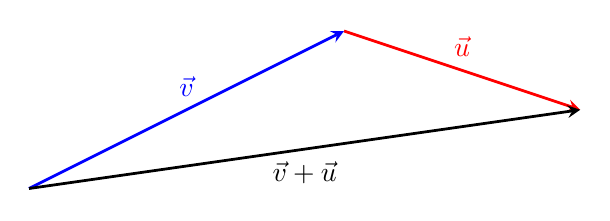
\begin{tikzpicture}
\draw[line width=1pt,-stealth,red](3,3)--(6,2);
\draw[line width=1pt,-stealth, blue](-1,1)--(3,3);
\draw[line width=1pt,-stealth](-1,1)--(6,2);

 \node[blue] at (1, 2.3)   (a) {$\vec{v}$};
 \node[red] at (4.5, 2.8)   (a) {$\vec{u}$};
  \node[black] at (2.5, 1.2)   (a) {$\vec{v}+\vec{u}$};
 \end{tikzpicture}
\end{center}
\end{expandable}


\begin{tikzpicture}[scale=1]
   \filldraw[teal, opacity=0.3](0,0)--(20,0)--(20,0.1)--(0,0.1)--cycle;
 \end{tikzpicture}

Length (norm, magnitude) of a vector

\begin{expandable}
  %  \begin{definition}
Let $\vec{v}=\begin{bmatrix}v_1\\ v_2\\ \vdots \\v_n\end{bmatrix}$ be a vector in $\RR^n$, then the \dfn{length}, or the \dfn{magnitude}, of $\vec{v}$ is given by
$$  \norm{\vec{v}}=\sqrt{v_1^2+v_2^2+\ldots +v_n^2}$$
%\end{definition}
\end{expandable}


\begin{tikzpicture}[scale=1]
   \filldraw[teal, opacity=0.3](0,0)--(20,0)--(20,0.1)--(0,0.1)--cycle;
 \end{tikzpicture}
 
Normal vector

\begin{expandable}
    A vector perpendicular to a plane is said to be a normal vector to the plane.
\end{expandable}


\begin{tikzpicture}[scale=1]
   \filldraw[teal, opacity=0.3](0,0)--(20,0)--(20,0.1)--(0,0.1)--cycle;
 \end{tikzpicture}
 
Orthogonal vectors

\begin{expandable}
 %   \begin{definition}
Let $\vec{u}$ and $\vec{v}$ be vectors in $\RR^n$. We say $\vec{u}$ and $\vec{v}$ are \dfn{orthogonal} if $\vec{u}\dotp \vec{v}=0$.
%\end{definition}
\end{expandable}


\begin{tikzpicture}[scale=1]
   \filldraw[teal, opacity=0.3](0,0)--(20,0)--(20,0.1)--(0,0.1)--cycle;
 \end{tikzpicture}
 
Parallel vectors

\begin{expandable}
    Two non-zero vectors are parallel if they are non-zero scalar multiples of each other.
\end{expandable}


\begin{tikzpicture}[scale=1]
   \filldraw[teal, opacity=0.3](0,0)--(20,0)--(20,0.1)--(0,0.1)--cycle;
 \end{tikzpicture}

Parallelogram rule for vector addition

\begin{expandable}
    \begin{center}
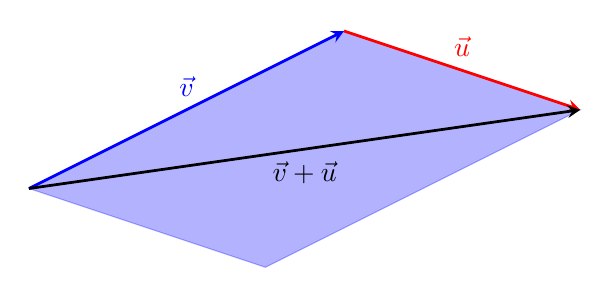
\begin{tikzpicture}
\filldraw[blue, opacity=0.3](-1,1)--(2,0)--(6,2)--(3,3)--cycle;
% \draw[line width=1pt,-stealth, blue](2,0)--(6,2);
  \draw[line width=1pt,red, -stealth](3,3)--(6,2);
 
%\draw[line width=1pt,-stealth,red](-1,1)--(2,0);
\draw[line width=1pt,-stealth, blue](-1,1)--(3,3);
\draw[line width=1pt,-stealth](-1,1)--(6,2);

 \node[blue] at (1, 2.3)   (a) {$\vec{v}$};

 \node[red] at (4.5, 2.8)   (a) {$\vec{u}$};
  \node[black] at (2.5, 1.2)   (a) {$\vec{v}+\vec{u}$};
  
 \end{tikzpicture}
\end{center}
\end{expandable}


\begin{tikzpicture}[scale=1]
   \filldraw[teal, opacity=0.3](0,0)--(20,0)--(20,0.1)--(0,0.1)--cycle;
 \end{tikzpicture}

Parametric equations of a line

\begin{expandable}
    Let $\vec{v}=\begin{bmatrix}v_1\\v_2\\\vdots\\v_n\end{bmatrix}$ be a direction vector for line $l$ in $\RR^n$, and let $(a_1, a_2,\ldots , a_n)$ be an arbitrary point on $l$.  Then the following parametric equations describe $l$:
\[
x_1=v_1t+a_1\]
\[x_2=v_2t+a_2\]
\[\vdots\]
\[x_n=v_nt+a_n
\]
\end{expandable}


\begin{tikzpicture}[scale=1]
   \filldraw[teal, opacity=0.3](0,0)--(20,0)--(20,0.1)--(0,0.1)--cycle;
 \end{tikzpicture}

Projection of a vector onto a vector

\begin{expandable}
    Let $\vec{v}$ be a vector, and let $\vec{d}$ be a non-zero vector.  The \dfn{projection of $\vec{v}$ onto $\vec{d}$} is given by 
$$\mbox{proj}_{\vec{d}}\vec{v}=\left(\frac{\vec{v}\dotp\vec{d}}{\norm{\vec{d}}^2}\right)\vec{d}$$
\end{expandable}


\begin{tikzpicture}[scale=1]
   \filldraw[teal, opacity=0.3](0,0)--(20,0)--(20,0.1)--(0,0.1)--cycle;
 \end{tikzpicture}

Pythagoras’ Theorem
\begin{expandable}
    You know the one!  Where have we used it in the context of points? vectors?
\end{expandable}


\begin{tikzpicture}[scale=1]
   \filldraw[teal, opacity=0.3](0,0)--(20,0)--(20,0.1)--(0,0.1)--cycle;
 \end{tikzpicture}

Scalar multiplication 

\begin{expandable}
    Let $\vec{u}=\begin{bmatrix}
u_1\\
u_2\\
\vdots\\
u_n
\end{bmatrix}$ be a vector in $\RR^n$, and let $k$ be a scalar, then
  $$k\vec{u}=k\begin{bmatrix}
u_1\\
u_2\\
\vdots\\
u_n
\end{bmatrix}=\begin{bmatrix}
ku_1\\
ku_2\\
\vdots\\
ku_n
\end{bmatrix}$$
\end{expandable}


\begin{tikzpicture}[scale=1]
   \filldraw[teal, opacity=0.3](0,0)--(20,0)--(20,0.1)--(0,0.1)--cycle;
 \end{tikzpicture}

Standard unit vectors

\begin{expandable}
    %\begin{definition}
  Let $\vec{e}_i$ denote a vector that has $1$ as the $i^{th}$ component and zeros elsewhere.  In other words, $$\vec{e}_i=\begin{bmatrix}
0\\
0\\
\vdots\\
1\\
\vdots\\
0
\end{bmatrix}$$ 
  where $1$ is in the $i^{th}$ position.  We say that  $\vec{e}_i$ is a \dfn{standard unit vector of $\RR^n$}.
%\end{definition}
\end{expandable}


\begin{tikzpicture}[scale=1]
   \filldraw[teal, opacity=0.3](0,0)--(20,0)--(20,0.1)--(0,0.1)--cycle;
 \end{tikzpicture}

Unit vector

\begin{expandable}
    A vector of length 1.
\end{expandable}


\begin{tikzpicture}[scale=1]
   \filldraw[teal, opacity=0.3](0,0)--(20,0)--(20,0.1)--(0,0.1)--cycle;
 \end{tikzpicture}

Vector

\begin{expandable}
    A quantity possessing magnitude and direction.
\end{expandable}


\begin{tikzpicture}[scale=1]
   \filldraw[teal, opacity=0.3](0,0)--(20,0)--(20,0.1)--(0,0.1)--cycle;
 \end{tikzpicture}

Vector addition

\begin{expandable}
  Let $\vec{u}=\begin{bmatrix}
u_1\\
u_2\\
\vdots\\
u_n
\end{bmatrix}$ and $\vec{v}=\begin{bmatrix}
v_1\\
v_2\\
\vdots\\
v_n
\end{bmatrix}$ be vectors in $\RR^n$.  We define $\vec{u}+\vec{v}$ by
  $$\vec{u}+\vec{v}=\begin{bmatrix}
u_1\\
u_2\\
\vdots\\
u_n
\end{bmatrix}+\begin{bmatrix}
v_1\\
v_2\\
\vdots\\
v_n
\end{bmatrix}=\begin{bmatrix}
u_1+v_1\\
u_2+v_2\\
\vdots\\
u_n+v_n
\end{bmatrix}$$
  \end{expandable}


\begin{tikzpicture}[scale=1]
   \filldraw[teal, opacity=0.3](0,0)--(20,0)--(20,0.1)--(0,0.1)--cycle;
 \end{tikzpicture}
  
Zero vector

\begin{expandable}
    A vector of zero length.  The zero vector has no direction.
\end{expandable}


\begin{tikzpicture}[scale=1]
   \filldraw[teal, opacity=0.3](0,0)--(20,0)--(20,0.1)--(0,0.1)--cycle;
 \end{tikzpicture}

\end{document}
